\section{Database}
\hspace*{0.7in} A database is an organized collection of data. The data are typically organized to model relevant aspects of reality in a way that supports processes requiring this information. For example, modeling the availability of rooms in hotels in a way that supports finding a hotel with vacancies. Database management systems (DBMSs) are specially designed software applications that interact with the user, other applications, and the database itself to capture and analyze data. A general-purpose DBMS is a software system designed to allow the definition, creation, querying, update, and administration of databases. Well-known DBMSs include MySQL, MariaDB, PostgreSQL, SQLite, Microsoft SQL Server, Oracle, SAP HANA, dBASE, FoxPro, IBM DB2, LibreOffice Base and FileMaker Pro. A database is not generally portable across different DBMSs, but different DBMSs can interoperate by using standards such as SQL and ODBC or JDBC to allow a single application to work with more than one database. \cite{1}\\
\hspace*{0.7in} Choosing between databases used to boil down to examining the differences between the available commercial and open source relational databases. The term "database" had become synonymous with SQL, and for a while not much else came close to being a viable solution for data storage. But recently there has been a shift in the database landscape. When considering options for data storage, there is a new game in town: NoSQL databases \cite{2}.

\section{NoSQL}
\hspace*{0.7in} NoSQL databases represent a recent evolution in enterprise application architecture, continuing the evolution of the past twenty years. In the 1990's, vertically integrated applications gave way to client-server architectures, and more recently, client-server architectures gave way to three-tier web application architectures. In parallel, the demands of web-scale data analysis added map-reduce processing into the mix and data architects started avoiding transactional consistency in exchange for incremental scalability and large-scale distribution. The NoSQL movement emerged out of this second ecosystem. NoSQL is often characterized by what it's not depending on whom you ask, it's either not only a SQL-based relational database management system or it's simply not a SQL-based RDBMS. While those definitions explain what NoSQL is not, they do little to explain what NoSQL is. Consider the fundamentals that have guided data management for the past forty years \cite{3}.\\
\hspace*{0.7in} In recent years there was a high demand for massively distributed databases with high partition tolerance but according to the CAP theorem it is impossible for a distributed system to simultaneously provide consistency, availability and partition tolerance guarantees. A distributed system can satisfy any two of these guarantees at the same time, but not all three. For that reason many NoSQL databases are using what is called eventual consistency to provide both availability and partition tolerance guarantees with a maximum level of data consistency. NewSQL is a class of modern relational databases that aims to provide the same scalable performance of NoSQL systems for online transaction processing (read-write) workloads while still using SQL and maintaining the ACID guarantees of a traditional database system. Such databases include Clustrix, EnterpriseDB, NuoDB and VoltDB \cite{1}.
\\
\hspace*{0.7in} The only thing that all NoSQL solutions providers generally agree on is that the term "NoSQL" isn't perfect, but it is catchy. Most agree that the "no" stands for "not only", an admission that the goal is not to reject SQL but, rather, to compensate for the technical limitations shared by the majority of relational database implementations. In fact, NoSQL is more a rejection of a particular software and hardware architecture for databases than of any single technology, language, or product. Relational databases evolved in a different era with different technological constraints, leading to a design that was optimal for the typical deployment prevalent at that time. But times have changed, and that once successful design is now a limitation. You might hear conversations suggesting that a better term for this category is NoRDBMS or half a dozen other labels, but the critical thing to remember is that NoSQL solutions started off with a different set of goals and evolved in a different environment, and so they are operationally different and, arguably, provide better suited solutions for many of today's data storage problems\cite{2}.
\\
\hspace*{0.7in} NoSQL emerged as companies, such as Amazon, Google, LinkedIn and Twitter struggled to deal with unprecedented data and operation volumes under tight latency constraints. Analyzing high-volume, real time data, such as web-site click streams, provides significant business advantage by harnessing unstructured and semi-structured data sources to create more business value. Traditional relational databases were not up to the task, so enterprises built upon a decade of research on distributed hash tables (DHTs) and either conventional relational database systems or embedded key/value stores, such as Oracle's Berkeley DB, to develop highly available, distributed key-value stores. Although some of the early NoSQL solutions built their systems atop existing relational database engines, they quickly realized that such systems were designed for SQL-based access patterns and latency demands that are quite different from those of NoSQL systems, so these same organizations began to develop brand new storage layers. In contrast, Oracle's Berkeley DB product line was the original key/value store; Oracle Berkeley DB Java Edition has been in commercial use for over eight years. By using Oracle Berkeley DB Java Edition as the underlying storage engine beneath a NoSQL system, Oracle brings enterprise robustness and stability to the NoSQL landscape.\cite{3}
\\
\hspace*{0.7in} The next generation of post-relational databases in the 2000s became known as NoSQL databases, including fast key-value stores and document-oriented databases. NoSQL databases are often very fast, do not require fixed table schemas, avoid join operations by storing denormalized data, and are designed to scale horizontally. The most popular NoSQL systems include MongoDB, Couchbase, Riak, memcached, Redis, CouchDB, Hazelcast, Apache Cassandra and HBase, which are all open-source software products.

\subsection{Why NoSQL}
\hspace*{0.7in} NoSQL databases first started out as in-house solutions to real problems in companies such as Amazon Dynamo, Google BigTable, LinkedIn Voldemort, Twitter FlockDB, Facebook Cassandra, Yahoo! PNUTS, and others. These companies didn't start off by rejecting SQL and relational technologies; they tried them and found that they didn't meet their requirements. In particular, these companies faced three primary issues: unprecedented transaction volumes, expectations of low-latency access to massive datasets, and nearly perfect service availability while operating in an unreliable environment. Initially, companies tried the traditional approach: they added more hardware or upgraded to faster hardware as it became available. When that didn't work, they tried to scale existing relational solutions by simplifying their database schema, de-normalizing the schema, relaxing durability and referential integrity, introducing various query caching layers, separating read-only from write-dedicated replicas, and, finally, data partitioning in an attempt to address these new requirements. Although each of these techniques extended the functionality of existing relational technologies, none fundamentally addressed the core limitations, and they all introduced additional overhead and technical tradeoffs. In other words, these were good band aids but not cures.\cite{2}
\\
\hspace*{0.7in} A major influence on the eventual design of NoSQL databases came from a dramatic shift in IT operations. When the majority of relational database technology was designed, the predominant model for hardware deployments involved buying large servers attached to dedicated storage area networks (SANs). Databases were designed with this model in mind: They expected there to be a single machine with the responsibility of managing the consistent state of the database on that system's connected storage. In other words, databases managed local data in files and provided as much concurrent access as possible given the machine's hardware limitations. Replication of data to scale concurrent access across multiple systems was generally unnecessary, as most systems met design goals with a single server and reliability goals with a hot stand-by ready to take over query processing in the event of master failure. Beyond simple failover replication, there were only a few options, and they were all predicated on this same notion of completely consistent centralized data management. Technologies such as two-phase commit and products such as Oracle's RAC were available, but they were hard to manage, very expensive, and scaled to only a handful of machines. Other solutions available included logical SQL statement-level replication, single-master multi-replica log-based replication, and other home-grown approaches, all of which have serious limitations and generally introduce a lot of administrative and technical overhead. In the end, it was the common architecture and design assumptions underlying most relational databases that failed to address the scalability, latency, and availability requirements of many of the largest sites during the massive growth of the Internet \cite{2}.
\\
\hspace*{0.7in} Given that databases were centralized and generally running on an organization's most expensive hardware containing its most precious information, it made sense to create an organizational structure that required at least a 1:1 ratio of database administrators to database systems to protect and nurture that investment. This, too, was not easy to scale, was costly, and could slow innovation. A growing number of companies were still hitting the scalability and performance wall even when using the best practices and the most advanced technologies of the time. Database architects had sacrificed many of the most central aspects of a relational database, such as joins and fully consistent data, while introducing many complex and fragile pieces into the operations puzzle. Schema devolved from many interrelated fully expressed tables to something much more like a simple key/value look-up. Deployments of expensive servers were not able to keep up with demand. At this point these companies had taken relational databases so far outside their intended use cases that it was no wonder that they were unable to meet performance requirements. It quickly became clear to them that they could do much better by building something in-house that was tailored to their particular workloads. These in-house custom solutions are the inspiration behind the many NoSQL products we now see on the market \cite{2}.
\\
\hspace*{0.7in} Furthermore, until recently, integrating NoSQL solutions with an enterprise application architecture required manual integration and custom development; Oracle's NoSQL Database provides all the desirable features of NoSQL solutions necessary for seamless integration into an enterprise application architecture \cite{3}.

\section{Types of NoSQL Databases}
\hspace*{0.7in} In isolation, NoSQL databases are enhanced for retrieve and append operations and also offer functionality beyond record storage. NoSQL databases shows their strong suit with regard to the elastic handling of variable data by document-oriented databases, the graph databases for representing relationships and in the reduction of a database to a container with KVpairs provided by key-value databases. \\
The four types of NoSQL Databases are as follows :
\begin{itemize}
  \item Graph Databases
  \item Document Databases
  \item Columnar Databses
  \item key-Values Stores
\end{itemize}

\subsection{Graph Databases}
\hspace*{0.7in} used which, again, can scale across multiple machines. NoSQL databases do not provide a high-level declarative query language like SQL to avoid overtime in processing. Rather, querying these databases is data-model specific. Many of the NoSQL platforms allow for RESTful interfaces to the data, while other offer query APIs. Examples are Neo4J, InfoGrid, Infinite Graph \cite{8}. Looking at the projection of domain models onto a data structure, there are two dominating schools - the relational way as used for RDBMS and graph and network structures, used for e.g. the Semantic Web. While graph structures in theory are normalizable even in RDBMS, this has serious query performance implications for recursive structures like for instance file trees and network structures like e.g. social graphs, due to the implementation characteristics of relational databases. Every operation over a relationship of a network results in a "join" operation in the RDBMS, implemented as a set-operation between the sets of primary keys for two tables - a slow operation and not scalable over growing numbers of tuples in these tables \cite{4}.
\\
\hspace*{0.7in} There is no existing general consensus on terminology regarding the area of graphs. There exist many different types of graph models. However, there is some effort to create the Property Graph Model, unifying most of the different graph implementations. According to it, information in a Property Graph is modeled using three basic building blocks:
\begin{itemize}
  \item node (a.k.a. vertex)
  \item relationship (a.k.a. edge) - with direction and Type (labeled and directed)
  \item property(a.k.a attribute) on nodes and relationships
\end{itemize}

\begin{figure}[h]
\centering
  % Requires \usepackage{graphicx}
  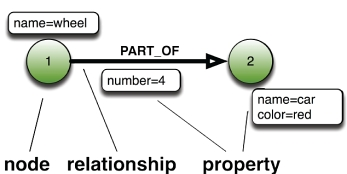
\includegraphics[width=10cm,height=6cm]{L1.jpg}
  \caption{Basic terminology for labeled property graphs}\label{Basic terminology for labeled property graphs}
\end{figure}

\begin{figure}[h]
\centering
  % Requires \usepackage{graphicx}
  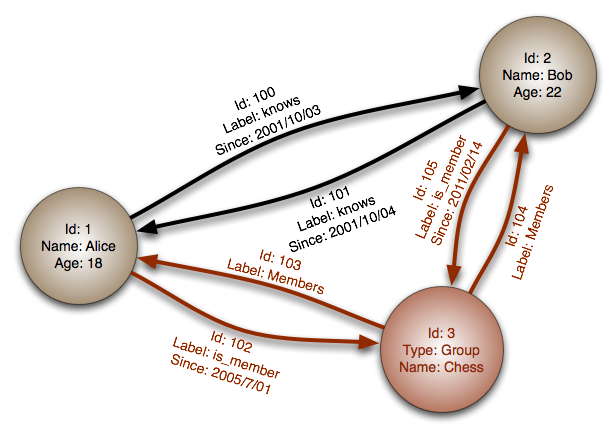
\includegraphics[width=10cm,height=8cm]{L2.png}
  \caption{labeled property graph.}\label{labeled property graph.}
\end{figure}

\begin{itemize}
  \item \textbf{For Example}
\end{itemize}
\hspace*{0.7in} As mentioned before, Social Networks represent just a tiny fraction of the applications of graph databases, as they are easy to understand for this example.
\\
\begin{figure}[h]
\centering
  % Requires \usepackage{graphicx}
  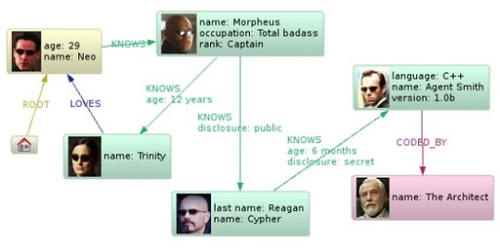
\includegraphics[width=10cm,height=8cm]{L3.jpg}
  \caption{Graph Database exapmle.}\label{Graph Database exapmle.}
\end{figure}
\\

\subsection{Document Databases}
\hspace*{0.7in} These were inspired by Lotus Notes and are similar to key-value stores. The model is basically versioned documents that are collections of other key-value collections. The semi-structured documents are stored in formats like JSON. Document databases are essentially the next level of Key/value, allowing nested values associated with each key.  Document databases support querying more efficiently. Examples are CouchDB, MongoDb \cite{8}. \\
\hspace*{0.7in} The central concept of a document-oriented database is the notion of a Document. While each document-oriented database implementation differs on the details of this definition, in general, they all assume documents encapsulate and encode data (or information) in some standard formats or encodings. Encodings in use include XML, YAML, JSON, and BSON, as well as binary forms like PDF and Microsoft Office documents (MS Word, Excel, and so on). Documents inside a document-oriented database are similar, in some ways, to records or rows in relational databases, but they are less rigid. They are not required to adhere to a standard schema, nor will they have all the same sections, slots, parts, or keys. For example, the following is a document:
$\{$ \\
\hspace*{0.4in} FirstName: "Bob", \\
\hspace*{0.4in} Address: "5 Oak St.", \\
\hspace*{0.4in} Hobby: "sailing" \\
$\}$
\\
\\
A second document might be: \\
\\
$\{$ \\
\hspace*{0.4in} FirstName: "Jonathan",  \\
\hspace*{0.4in} Address: "15 Wanamassa Point Road", \\
\hspace*{0.4in} Children: [ \\
\hspace*{0.4in} $\{$Name: "Michael", Age: 10$\}$,   \\
\hspace*{0.4in} $\{$Name: "Jennifer", Age: 8$\}$,   \\
\hspace*{0.4in} $\{$Name: "Samantha", Age: 5$\}$,   \\
\hspace*{0.4in} $\{$Name: "Elena", Age: 2$\}$   \\
\hspace*{0.4in} ]   \\
$\}$    \\
\\
\hspace*{0.7in} These two documents share some structural elements with one another, but each also has unique elements. Unlike a relational database where every record contains the same fields, leaving unused fields empty; there are no empty 'fields' in either document (record) in the above example. This approach allows new information to be added to some records without requiring that every other record in the database share the same structure \cite{5}.
\subsection{Columnar Databases}
\hspace*{0.7in} These were created to store and process very large amounts of data distributed over many machines. There are still keys but they point to multiple columns. The columns are arranged by column family. Examples are Cassandra, HBase \cite{8}. \\
A column family is a NoSQL object that contains columns of related data. It is a tuple (pair) that consists of a key-value pair, where the key is mapped to a value that is a set of columns. In analogy with relational databases, a column family is as a "table", each key-value pair being a "row". Each column is a tuple (triplet) consisting of a column name, a value, and a timestamp. In a relational database table, this data would be grouped together within a table with other non-related data \cite{6}.\\
Two types of column families exist:
\begin{itemize}
  \item Standard column family: contains only columns
  \item Super column family: contains a map of super columns.
\end{itemize}

\subsection{Key-Value Store Databases}
\hspace*{0.7in} The main idea here is using a hash table where there is a unique key and a pointer to a particular item of data. The Key/value model is the simplest and easiest to implement. But it is inefficient when you are only interested in querying or updating part of a value, among other disadvantages. Examples: Tokyo Cabinet/Tyrant, Redis, Voldemort, Oracle BDB, Amazon SimpleDB, Riak \cite{8}.
\\
\hspace*{0.7in} Key-value stores allow the application to store its data in a schema-less (key, value) pairs. This data is stored in a hash table like data-types, so that each value can be accessed by its major or minor key. Even though such storage facility might not be much effective as they provide single way to access the values, but excludes the need for a fixed data model.
\\
\begin{figure}[h]
\centering
  % Requires \usepackage{graphicx}
  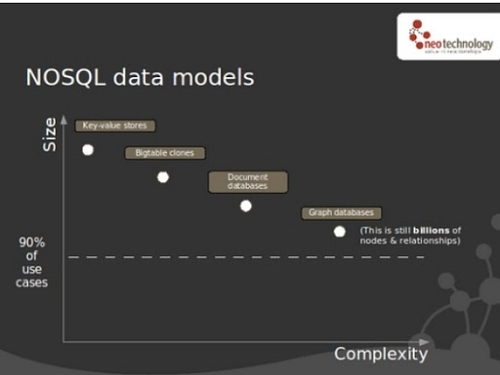
\includegraphics[width=10cm,height=8cm]{L4.jpg}
  \caption{NoSQL Data Models}\label{NoSQL Data Models}
\end{figure}
\\

\subsubsection{Oracle Key Value Pair NoSQL Database}
\hspace*{0.7in} Oracle NoSQL Database provides multi-terabyte distributed key/value pair storage that offers scalable throughput and performance. That is, it services network requests to store and retrieve data which is organized into key-value pairs. Oracle NoSQL Database services these types of data requests with a latency, throughput, and data consistency that is predictable based on how the store is configured. Oracle NoSQL Database offers full Create, Read, Update and Delete (CRUD) operations with0 adjustable durability guarantees. Oracle NoSQL Database is designed to be highly available, with excellent throughput and latency, while requiring minimal administrative interaction. \\
\hspace*{0.7in} Oracle NoSQL Database provides performance scalability. If you require better performance, you use more hardware. If your performance requirements are not very steep, you can purchase and manage fewer hardware resources. Oracle NoSQL Database is meant for any application that requires network-accessible key-value data with user-definable read/write performance levels. The typical application is a web application which is servicing requests across the traditional three-tier architecture: web server, application server, and back-end database. In this configuration, Oracle NoSQL Database is meant to be installed behind the application server, causing it to either take the place of the back-end database, or work alongside it. To make use of Oracle NoSQL Database, code must be written (using Java or C) that runs on the application server. An application makes use of Oracle NoSQL Database by performing network requests against Oracle NoSQL Database's key-value store, which is referred to as the KVStore. The requests are made using the Oracle NoSQL Database Driver, which is linked into your application as a Java library (.jar file), and then accessed using a series of Java APIs. \\
\begin{itemize}
    \item The KVStore :
\end{itemize}
\hspace*{0.7in} The KVStore is a collection of Storage Nodes which host a set of Replication Nodes. Data is spread across the Replication Nodes. The store contains multiple Storage Nodes. Every Storage Node hosts one or more Replication Nodes as determined by its capacity. \\
\begin{itemize}
    \item Replication Nodes and Shards :
\end{itemize}
\hspace*{0.7in} At a very high level, a Replication Node can be thought of as a single database which contains key-value pairs. Replication Nodes are organized into shards. A shard contains a single Replication Node, called the master node, which is responsible for performing database writes. The master node copies those writes to the other Replication Nodes in the shard, called the replicas. These replicas obtain a full copy of the data from the corresponding master node and are used to service read-only operations. Although there can be only one master node at any given time, any of the members of the shard are capable of becoming a master node.
\\
\begin{itemize}
    \item Replication Factor :
\end{itemize}
\hspace*{0.7in} The number of nodes belonging to a shard is called its Replication Factor. The larger a shard's Replication Factor, the faster its read throughput (because there are more machines to service the read requests) but the slower its write performance (because there are more machines to which writes must be copied).
\\
\begin{itemize}
    \item Partitions :
\end{itemize}
\hspace*{0.7in} Each shard contains one or more partitions. Key-value pairs in the store are organized according to the key. Keys, in turn, are assigned to a partition. Once a key is placed in a partition, it cannot be moved to a different partition.
\\
\begin{itemize}
    \item KVLite :
\end{itemize}
\hspace*{0.7in} KVLite is a simplified version of Oracle NoSQL Database. It provides a single-node store that is not replicated. It runs in a single process without requiring any administrative interface. You configure, start, and stop KVLite using a command line interface.

\begin{itemize}
    \item Architecture of Key Value Pair NoSQL Database
\end{itemize}

\begin{figure}[h]
\centering
  % Requires \usepackage{graphicx}
  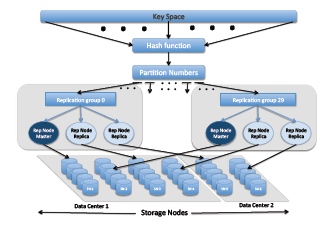
\includegraphics[width=10cm,height=8cm]{A1.png}
  \caption{Architecture of Key Value Pair NoSQL Database}
  \label{Architecture of Key Value Pair NoSQL Database}
\end{figure}

\begin{itemize}
    \item The CAP Theorem of NoSQL Database
\end{itemize}
\hspace*{0.7in} Despite the high demand in recent years for massively distributed databases with high partition fault-tolerance, the CAP theorem stipulates that it is actually impossible for a distributed system to provide consistency, availability and partition fault-tolerance guarantees simultaneously; a distributed system can satisfy at most any two of these guarantees at the same time, but not all three. These guarantees can be understood as follows:
\\
\begin{figure}[h]
\centering
  % Requires \usepackage{graphicx}
  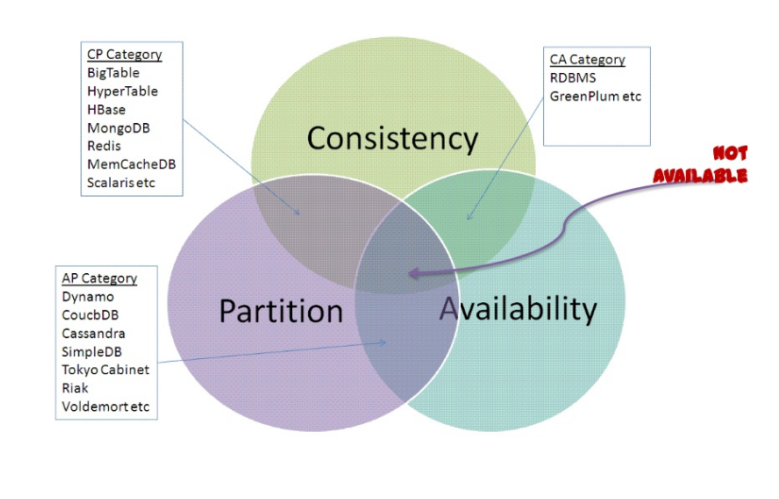
\includegraphics[width=10cm,height=8cm]{C1.png}
  \caption{CAP Theorem of NoSQL}\label{CAP Theorem of NoSQL}
\end{figure}
\\
\textbf{Consistency }: Concurrently executing queries see the same valid and consistent data at the same time. \\
\textbf{Availability }: This is a guarantee that every request receives a response about whether it succeeded or failed. \\
\textbf{Partition-tolerance }: Also known as fault-tolerance, this is a guarantee that the system continues to operate despite arbitrary message loss.\\

\hspace*{0.7in} Because no distributed system is capable of satisfying all three guarantees at the same time, a trade-off must be made. While traditional databases make that decision for us, NoSQL databases provide these guarantees as tuning options. Database vendors must always decide which two to prioritize. The options are as follows:
\begin{enumerate}
  \item Availability is compromised in favour of consistency and partition-tolerance.
  \item Partition-tolerance is forfeited in favour of consistency and availability.
  \item Consistency is compromised but systems are always available and can work when parts are partitioned.
\end{enumerate}

Traditional SQL databases place a high priority on consistency and fault-tolerance and have generally as a result chosen to go with the first option above and forfeit high availability. NoSQL databases frequently leave that decision to the application operations team and provide configuration options so that the preferred options can be chosen based on the application use case

\begin{itemize}
    \item NoSQL in Practice
\end{itemize}
There are many products that now claim to be part of the NoSQL database market, far too many to mention here or describe in any detail.
\\
\begin{figure}[h]
\centering
  % Requires \usepackage{graphicx}
  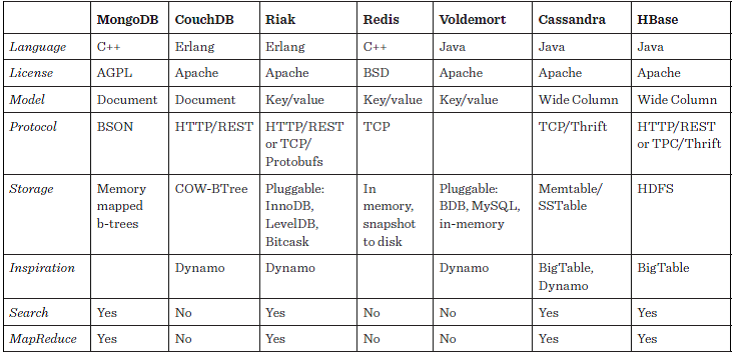
\includegraphics[width=13cm,height=7cm]{T1.png}
  \caption{NoSQL in Practice}\label{NoSQL in Practice}
\end{figure}

\section{Characteristics of NoSQL Databases}
\begin{itemize}
  \item Auto-sharding - A NoSQL database automatically spreads data across servers, without requiring applications to participate. Servers can be added or removed from the data layer without application downtime, with data (and I/O) automatically spread across the servers. Most NoSQL databases also support data replication, storing multiple copies of data across the cluster, and even across data centers, to ensure high availability and support disaster recovery. A properly managed NoSQL database system should never need to be taken offline, for any reason, supporting 24x365 continuous operations of applications.

  \item Unstructured Database.

  \item Distributed query support - "Sharding" a relational database can reduce, or eliminate in certain cases, the ability to perform complex data queries. NoSQL database systems retain their full query expressive power even when distributed across hundreds of servers.

  \item Integrated caching - To reduce latency and increase sustained data throughput, advanced NoSQL database technologies transparently cache data in system memory. This behavior is transparent to the application developer and the operations team, compared to relational technology where a caching tier is usually a separate infrastructure tier that must be developed to, deployed on separate servers, and explicitly managed by the ops team.
\end{itemize}